%
%
%
\clearpage
\section{Characterization of electromagnetic shower properties with
a sampling calorimeter}
\label{sec:emshowerproperties}

\FIXME{Add introduction}

%%
%%
%%
\subsection{Longitudinal evolution and energy estimation}
\label{subsec:longevol}

In order to characterize the longitudinal evolution of the showers in
our setup we count the total energy deposited by all hits in the Si layers. 
Energy is measured relatively to the estimated MIP signal (see details
ahead in Sec.~\ref{sec:digi}).
In this study electron events are used: for incoming energies
below 150\GeV, 2500 events have been generated; for higher energies
1250 events are used.

Figure~\ref{fig:showerfits} shows the longitudinal shower evolution
for single electron events as function of the \Xnot transversed in the
detector.
It can be observed that the level of energy fluctuations for low
energetic electrons is non-negligible, with $\delta$ deposits
dominating the contribution to the total energy deposited in each Si
layer.
For sufficiently energetic electrons these contributions become of
second order and the characterization of the shower is dominated by
the statistical fluctuations in the number of particles comprising the shower.
For very high energy showers ($>$150\GeV) part of the energy can't be
contained in the detector setup using 25\Xnot. Given that in this
regime the showers are dominated by statistical fluctuations in its
composition a fit to the longitudinal profile can be used safely and
used to estimate the leakage fraction.

\begin{figure}[h!]
  \begin{center}
    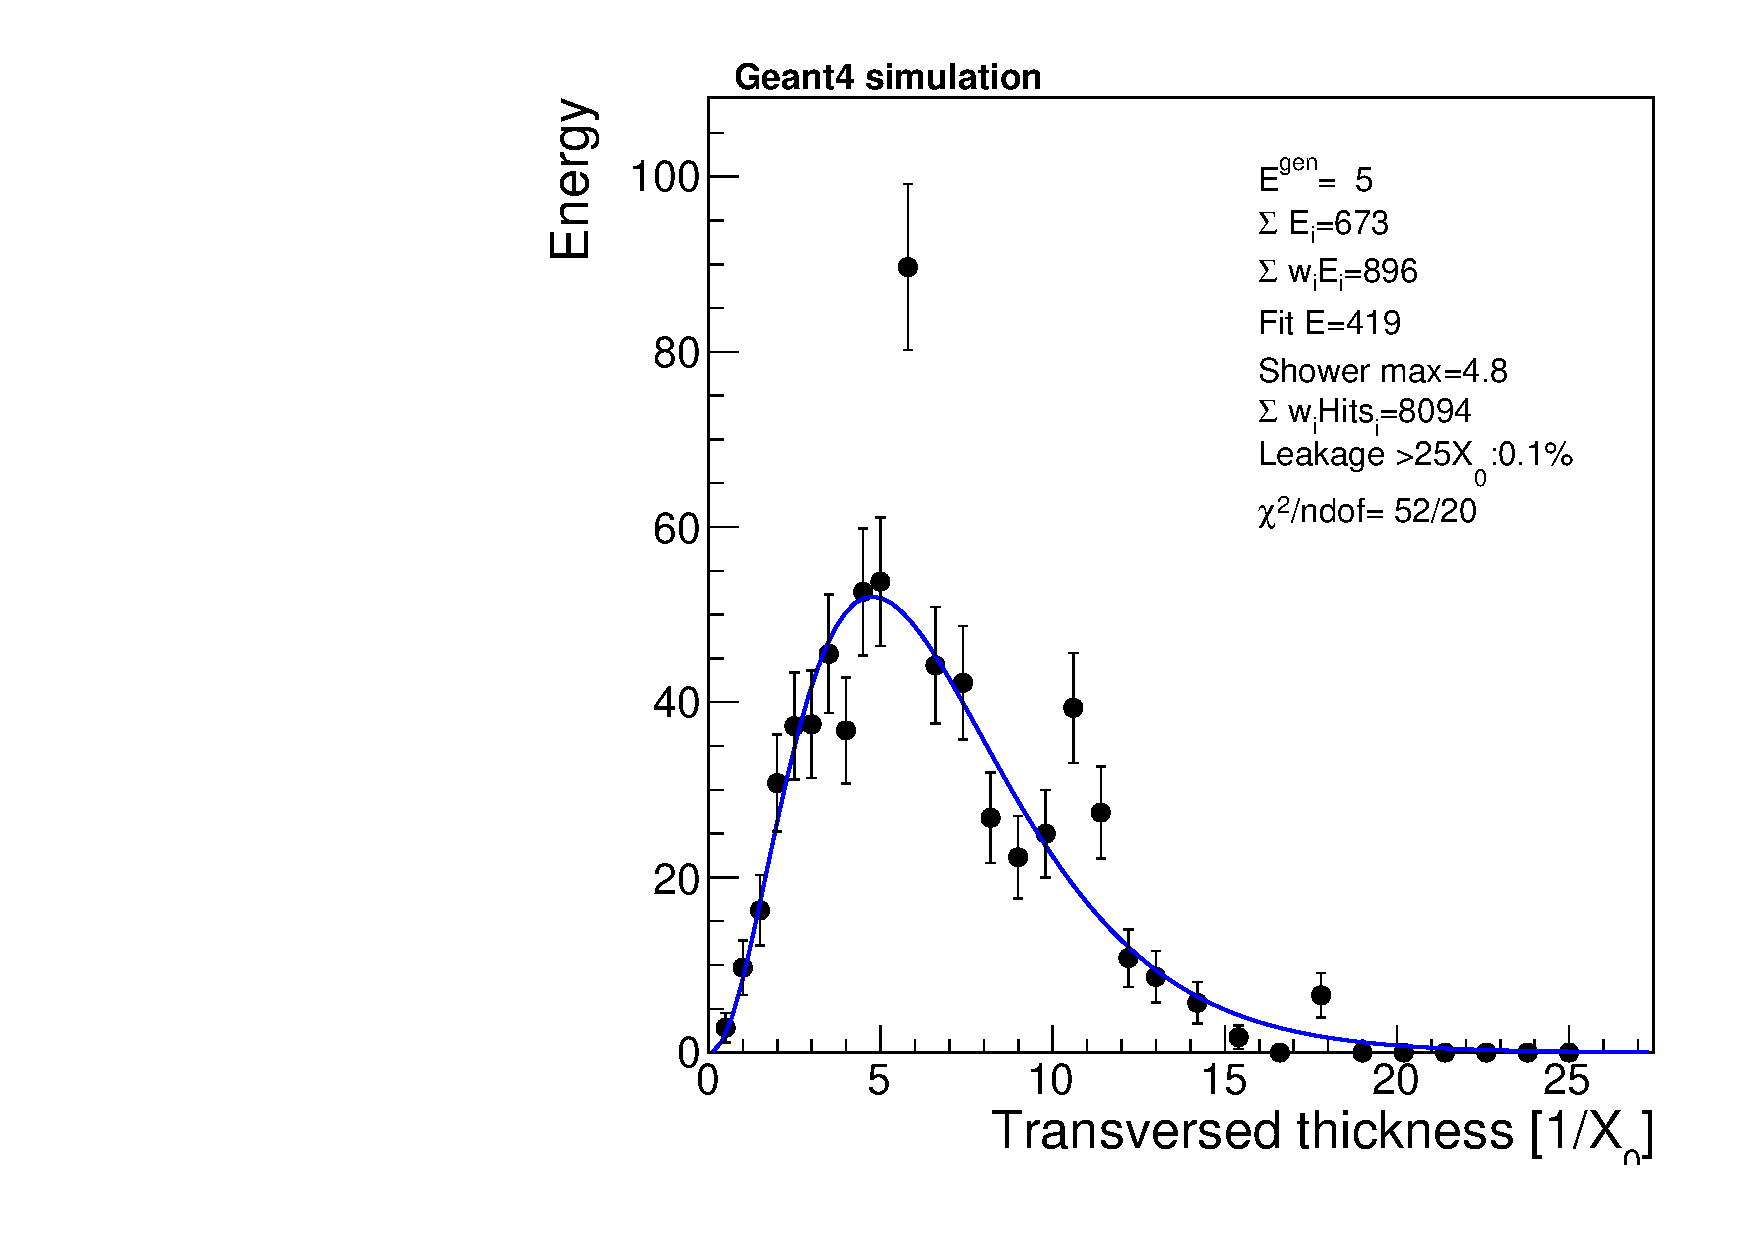
\includegraphics[width=0.24\textwidth]{figures/version_3e_5_5_showerfits}
    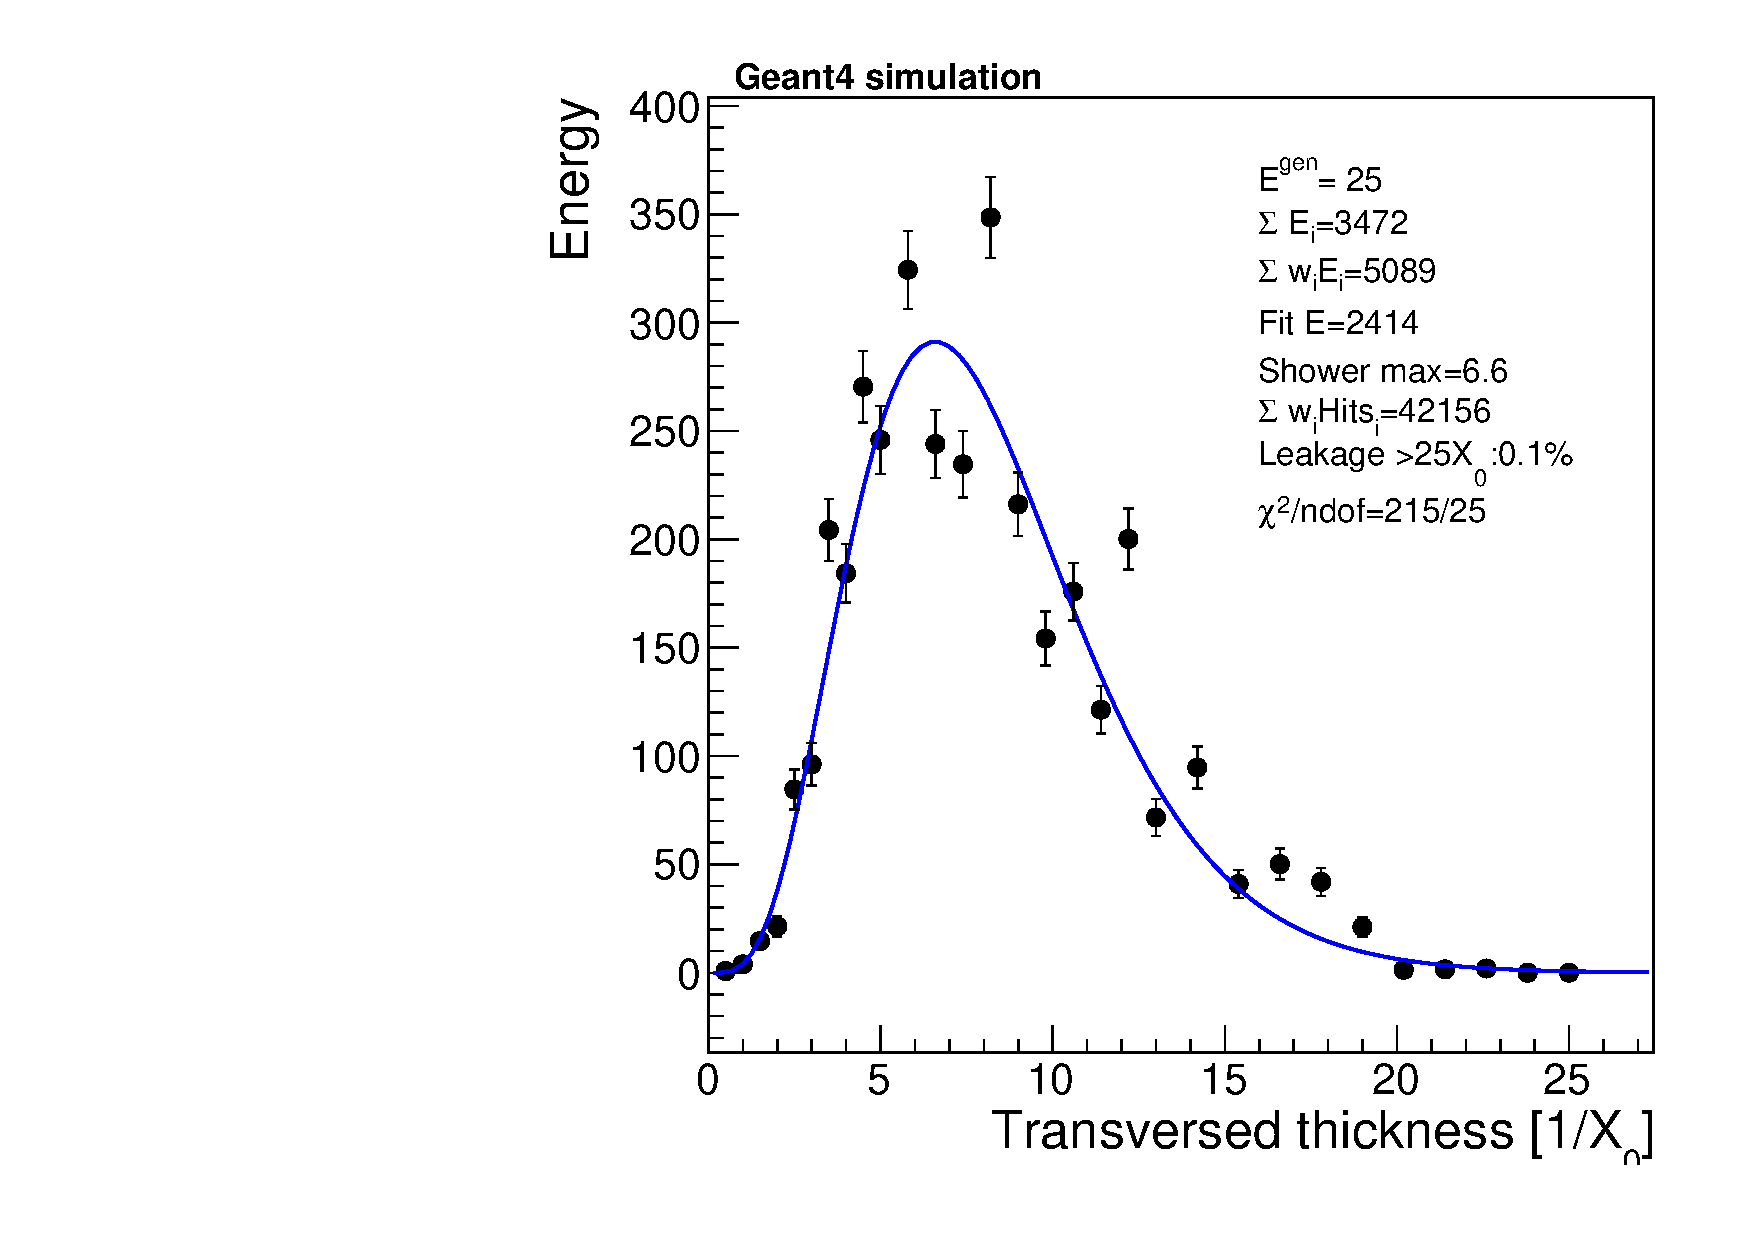
\includegraphics[width=0.24\textwidth]{figures/version_3e_25_8_showerfits}
    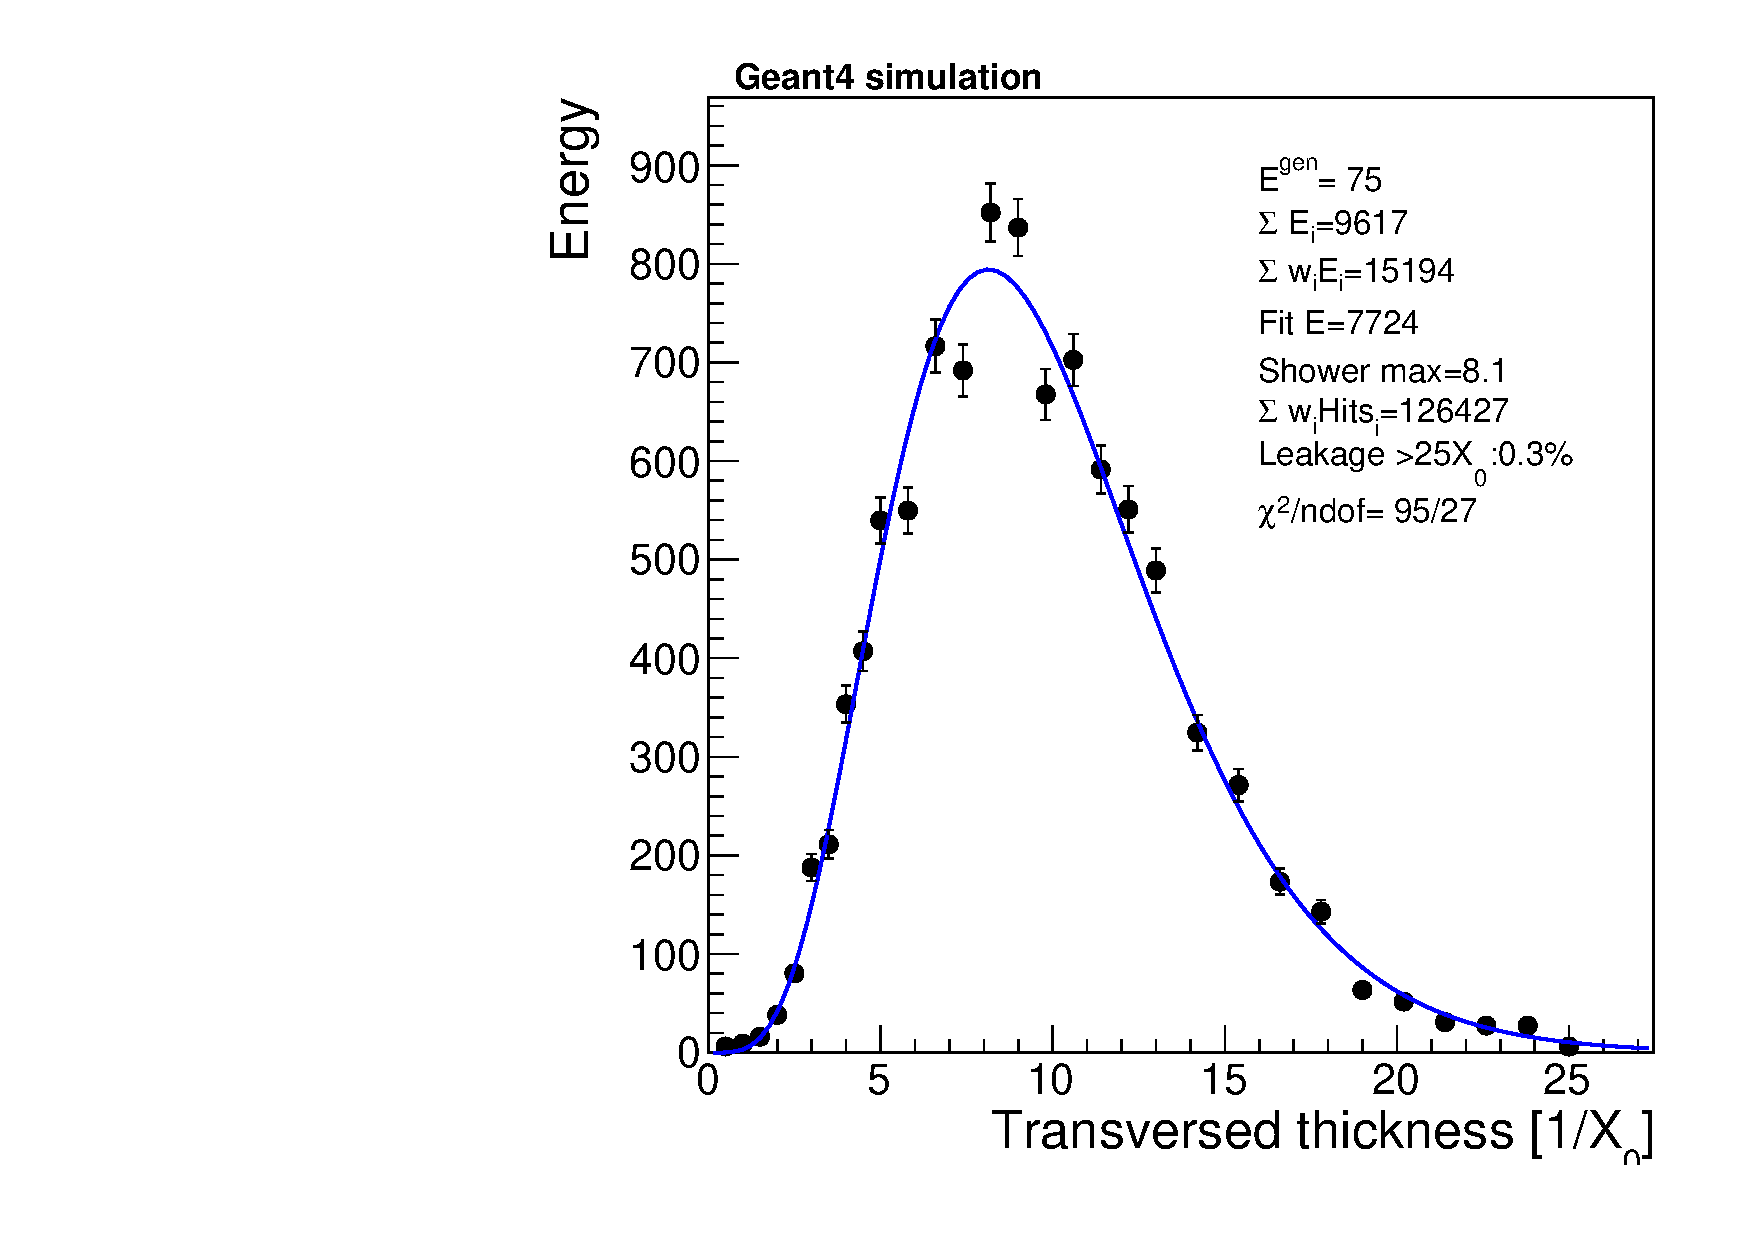
\includegraphics[width=0.24\textwidth]{figures/version_3e_75_6_showerfits}
    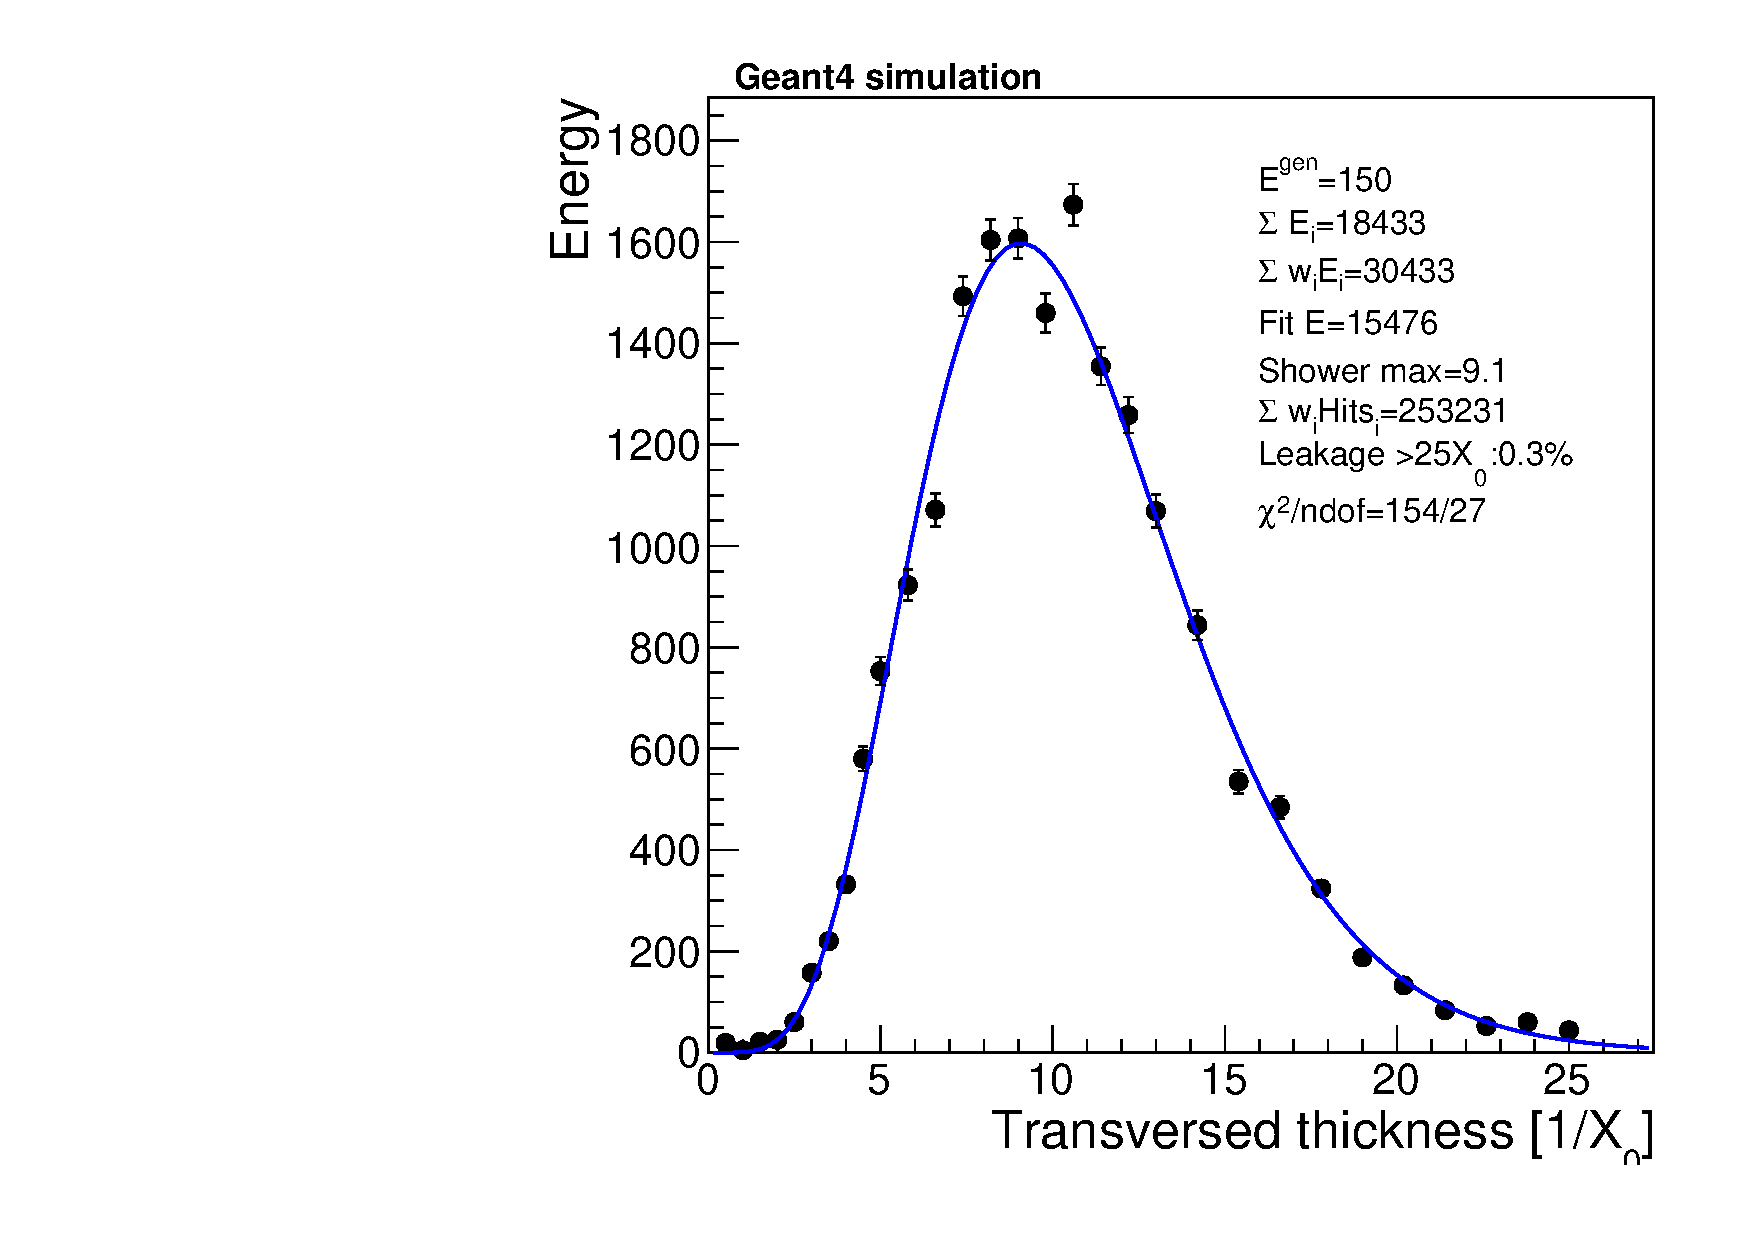
\includegraphics[width=0.24\textwidth]{figures/version_3e_150_6_showerfits}
    \caption{From {\em left} to {\em right}: energy deposits in different Si layers for single
      electron events with energies: 10, 25, 50, 100\GeV. The deposits
    are shown as function of the transversed distance in \Xnot
    units. A fit is overlaid using the functional form described in
    the text. 
     The results obtained for the different energy estimators
     considered in the analysis, as well as for the shower leakage
     estimated from the fit, are shown in the caption}
    \label{fig:showerfits}
  \end{center}
\end{figure}

Thus, different methods to estimate the total energy of the shower are
compared:

\begin{description}

\item[Raw energy] we sum inclusively of all the energy deposited in
  the Si layers assuming the full sensitive area volume;

\item[Weighted energy] we sum the energy deposited in each Si layer
  normalized by the material overburden of the sampling section,\ie:

\begin{equation}
{\rm weighted~E}=\sum_{i=1}^{N} \frac{X_0^i}{X_0^1}\cdot E_i
\label{eq:weightenest}
\end{equation}

For the baseline setup these weights correspond to 1 for section A,
1.6 for section B and 2.4 for section B.
These weights can also be optimised to minimise the energy resolution
for the incoming energy range of interest.

\item[Shower profile fit] - a functional form is used to adjust the
  measured energy deposits in each layer:

\begin{equation}
\mathcal{E}(x)=\alpha\cdot x^{a} \cdot e^{-bx} 
\label{eq:showerprof}
\end{equation}

where x is the transversed material overburden measured in \Xnot
units. This approach is expected to recover the shower leakage for
higher incident energies.

\item[Shower maximum] - the position of the shower max can be used as a
  coarse estimator for the energy. It can be estimated after the
  shower fit by the ratio $X_{0}^{\max}=b/a$.

\item[Hit counting] - this estimator, altough impossible to be used in
  reality, is used to gauge to potential of the setup. We use the
  weighted sum  of the number of hits generated per Si layer as an
  estimator of the initial energy. The weights are the same as define
  in Eq.~\ref{eq:weightenest}.

\end{description}

For each method the distribution of the estimator is fitted with a
gaussian for each incoming generated beam energy. An unbinned fit is
used for this purpose. Figures~\ref{fig:fithitcount}
and~\ref{fig:fitwen}
show two examples using the weighted energy and the hit counting
estimators correspondingly.

\begin{figure}[h!]
  \begin{center}
    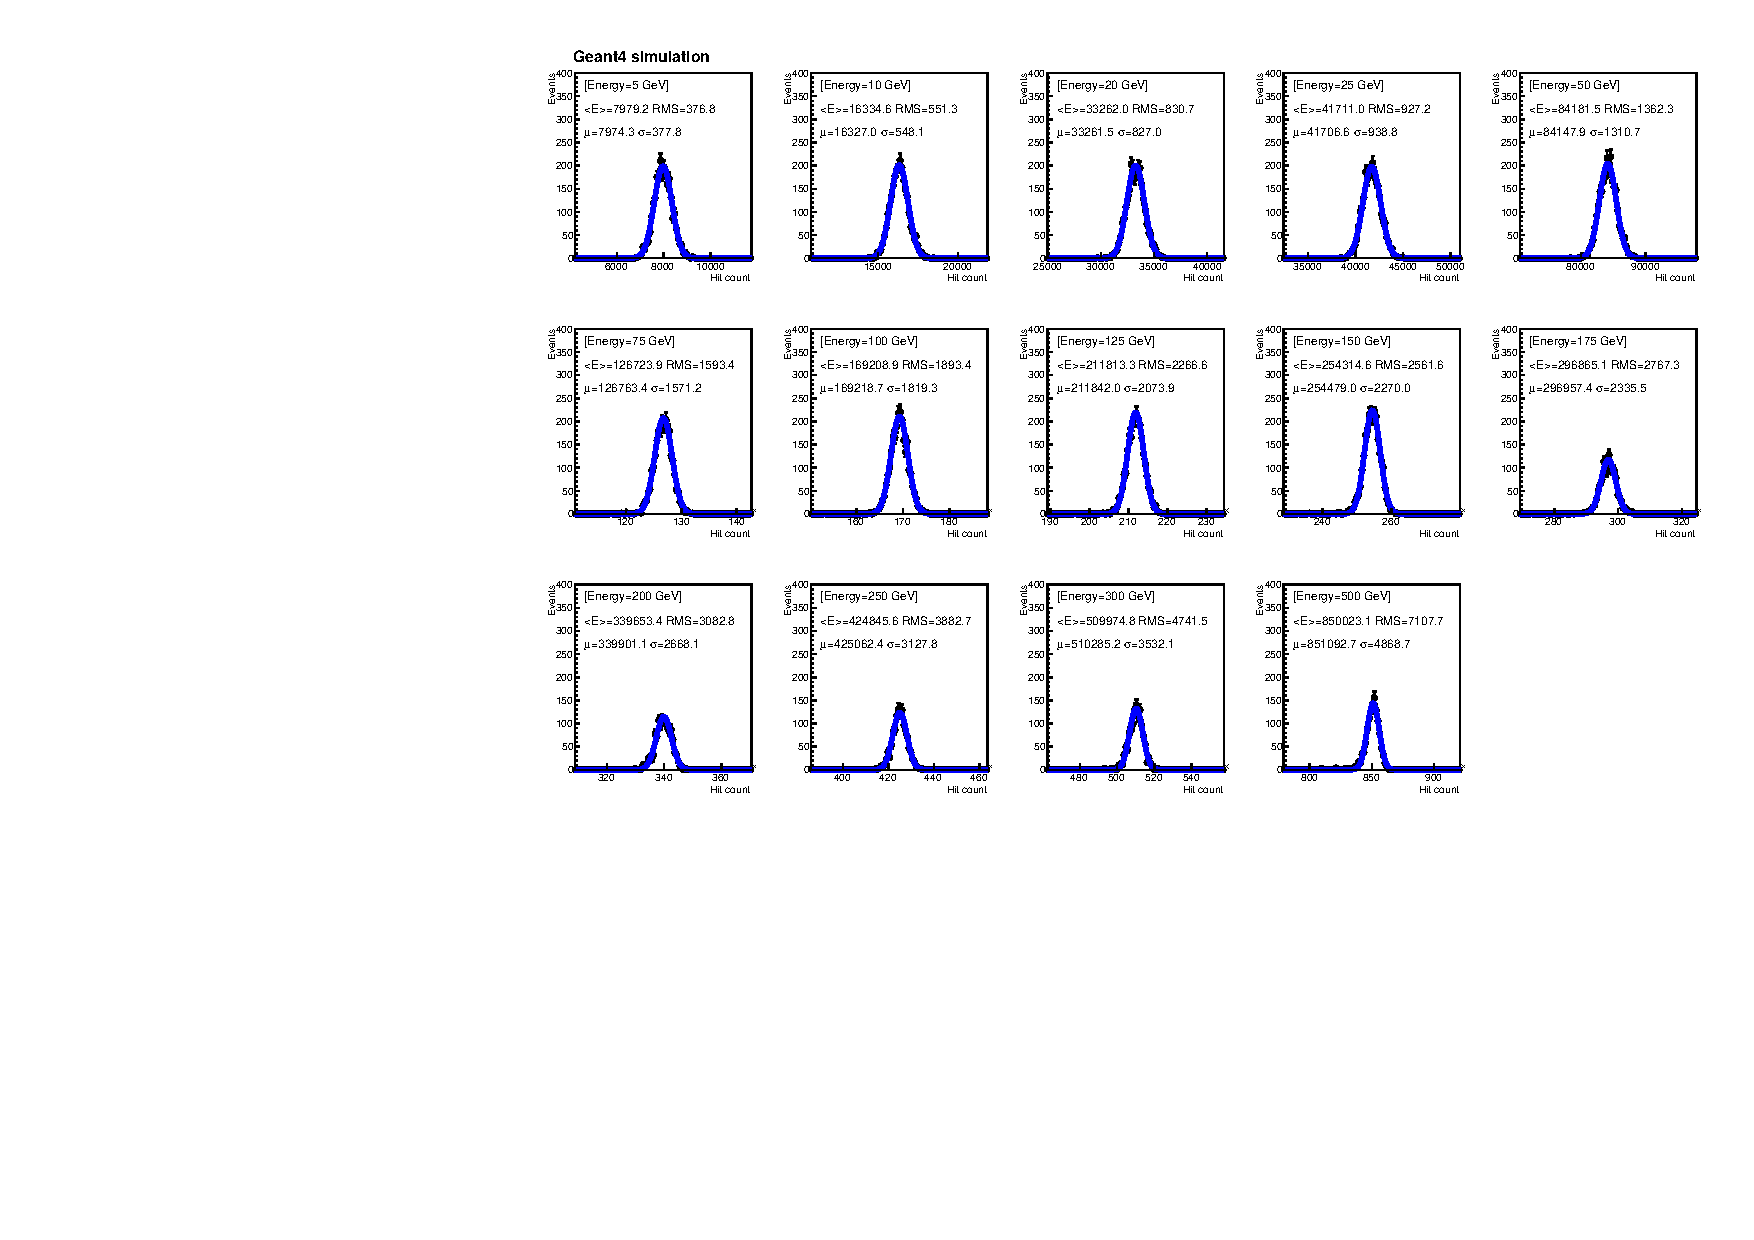
\includegraphics[width=0.99\textwidth]{figures/recenergy_nemHits}
    \caption{Weighted energy sum estimator distributions for different
    beam energies. The result of an unbinned gaussian fit is
    superimposed and the mean and average of the distribution and the
    gaussian are compared in the caption.}
    \label{fig:fithitcount}
  \end{center}
\end{figure}

\begin{figure}[h!]
  \begin{center}
    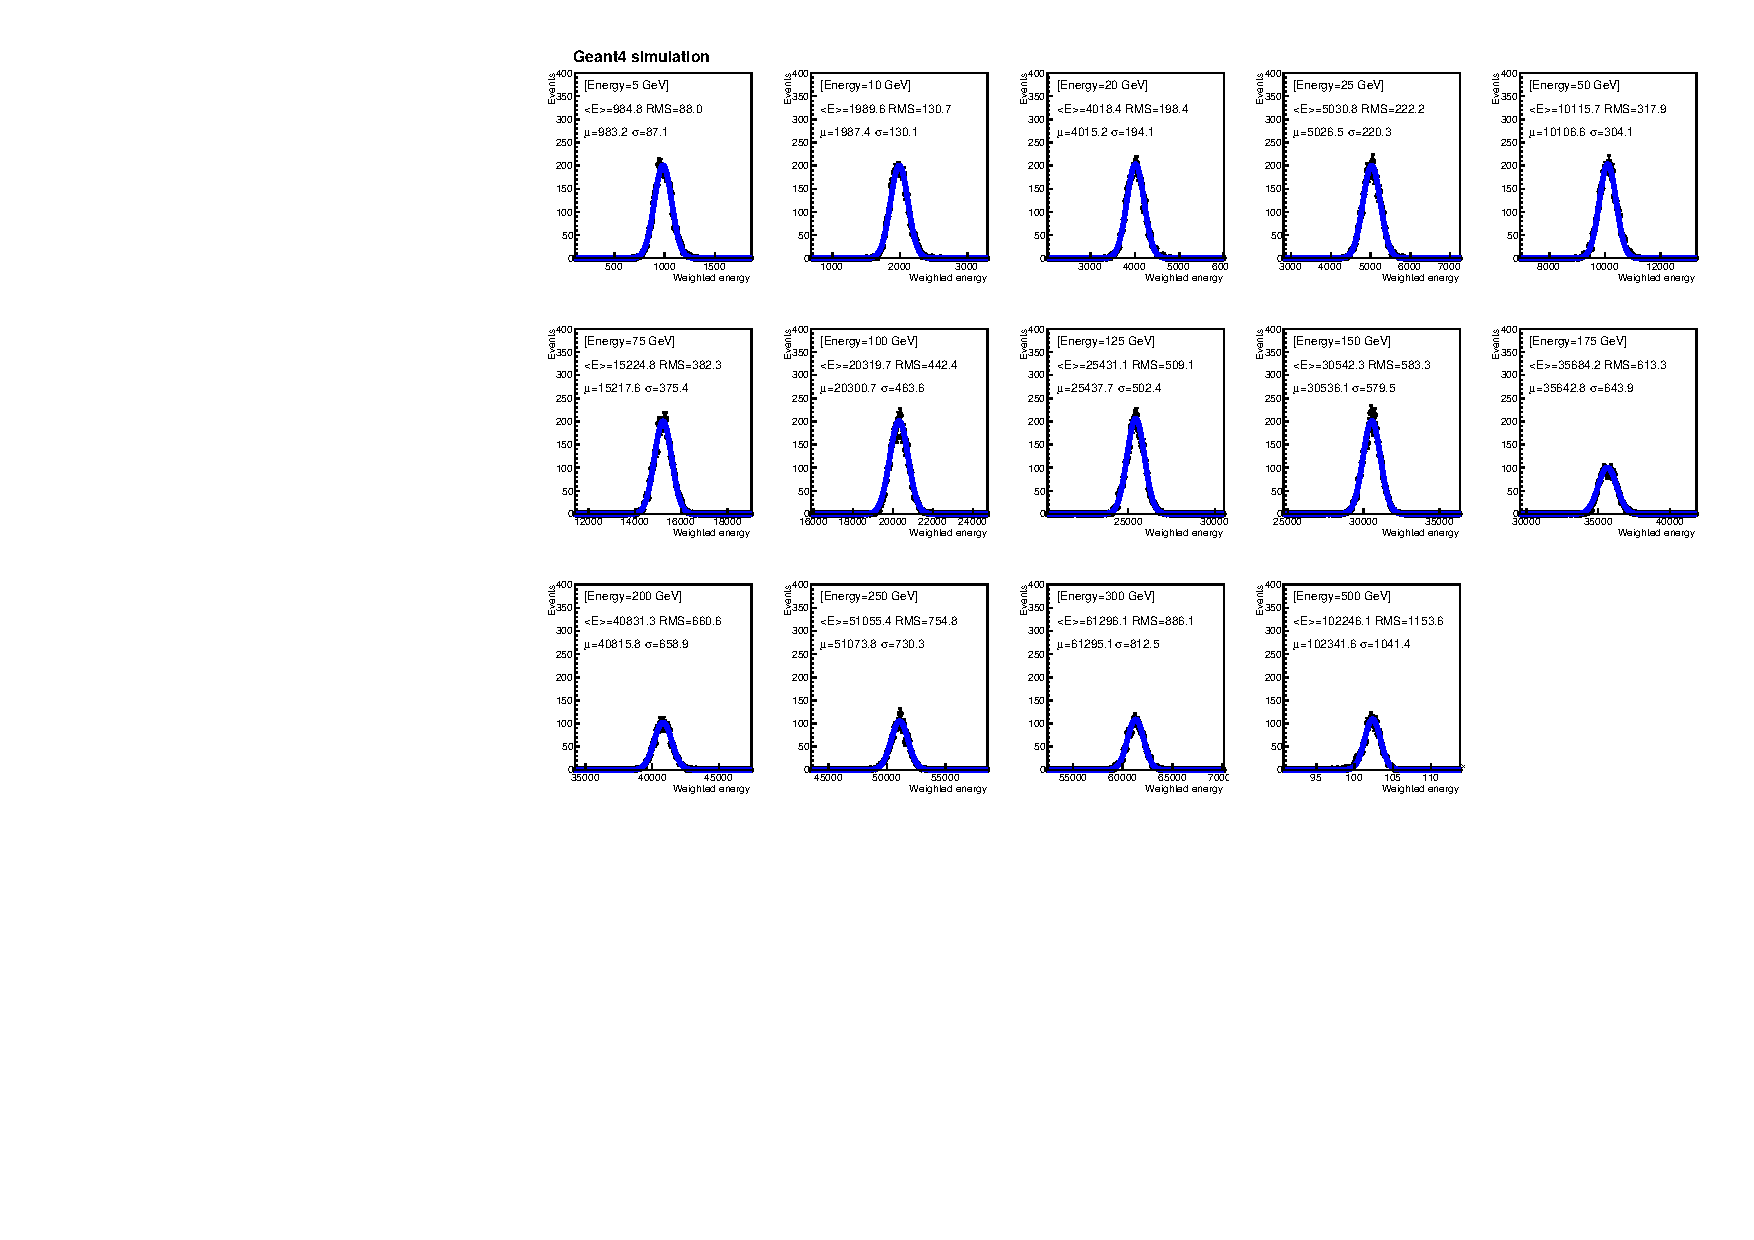
\includegraphics[width=0.99\textwidth]{figures/recenergy_sumWEn}
    \caption{Similar to Fig.~\ref{fig:fithitcount} for the weighted energy sum estimator.}
    \label{fig:fitwen}
  \end{center}
\end{figure}

The parameters of the fitted gaussians can be used for two purposes:
the mean is used to obtain the calibration (\ie dependency of the
energy estimator on the incoming energy) and the ratio of the width
with respect to the mean as an estimator for the resolution.
The calibration curves obtained are shown in Fig.~\ref{fig:baselinelinandresol}
{\em left} where linear behaviour is observed for all the estimators.
Figure~\ref{fig:baselinelinandresol} {\em right} shows the energy
resolution as a function of the incoming energy. 
A fit to a resolution model is super-imposed for each curve. The
resolution model is based on the quadratic sum of a stochastic term
(proportional to $1/\sqrt{E}$) with a constant term,\ie:

\begin{equation}
\left(\frac{\sigma_{\rm E}}{\rm E}\right)^2 = \left(\frac{\sigma_{\rm
      stoch}}{\sqrt{\rm E}}\right)^2+\sigma_{\rm cte}^2
\label{eq:resmodel}
\end{equation}

As expected, altough the raw energy estimator scales faster with
energy (\ie has smaller stochastic term) its resolution fastly
saturates at a non-negligible due to the fact that the sampling is
non-uniform. The weighted energy estimator is able to recover from
this attaining a baseline resolution of the order of 20.9\%. The
residual constant term can be almost fully removed with a shower
leakage recovery algorithm such as the one provided by the fitted
energy estimator - in this approach the constant term is observed to
be compatible with 0.
The hit count approach yields the best resolution expected to be
attainable with this setup. The shower max estimator has worse
resolution and large constant term.

\begin{figure}[h!]
  \begin{center}
   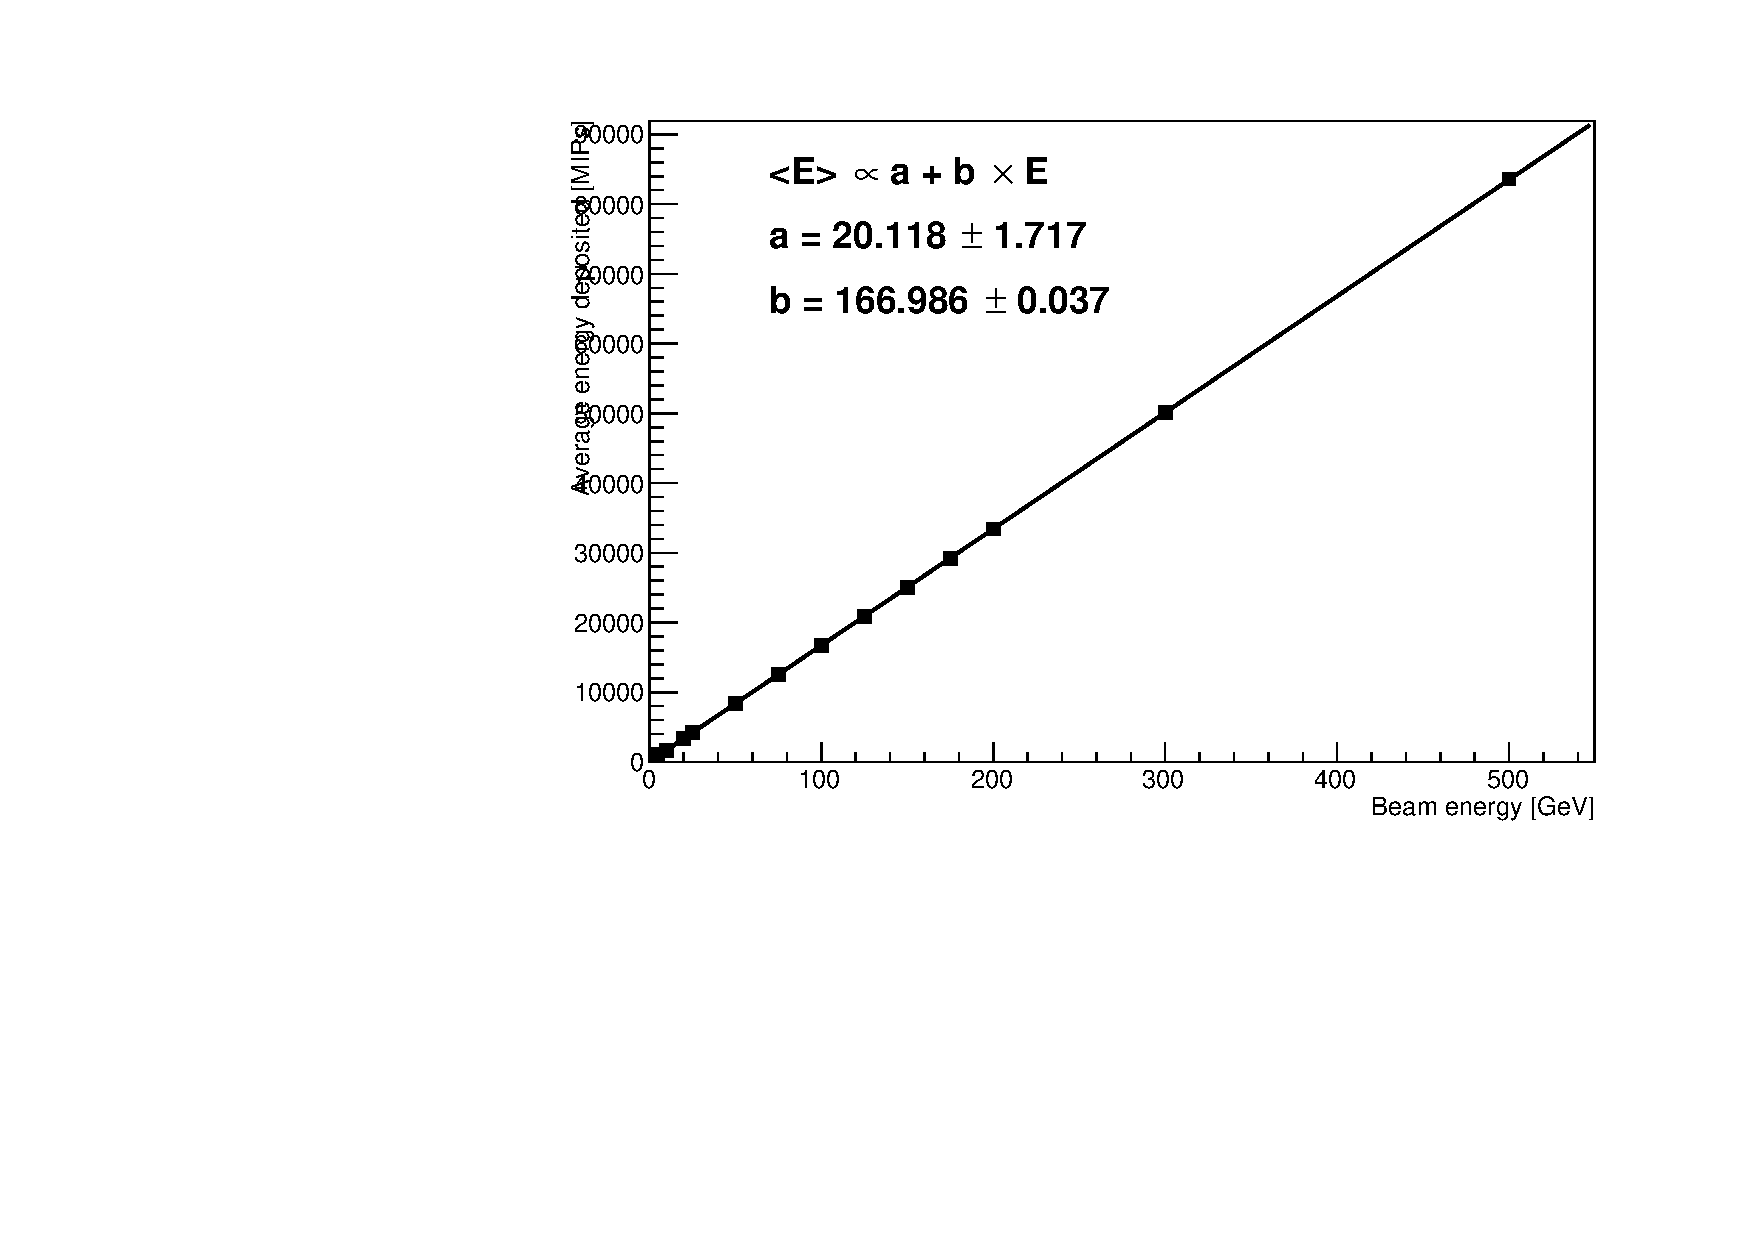
\includegraphics[width=0.48\textwidth]{figures/e_calibFit}
    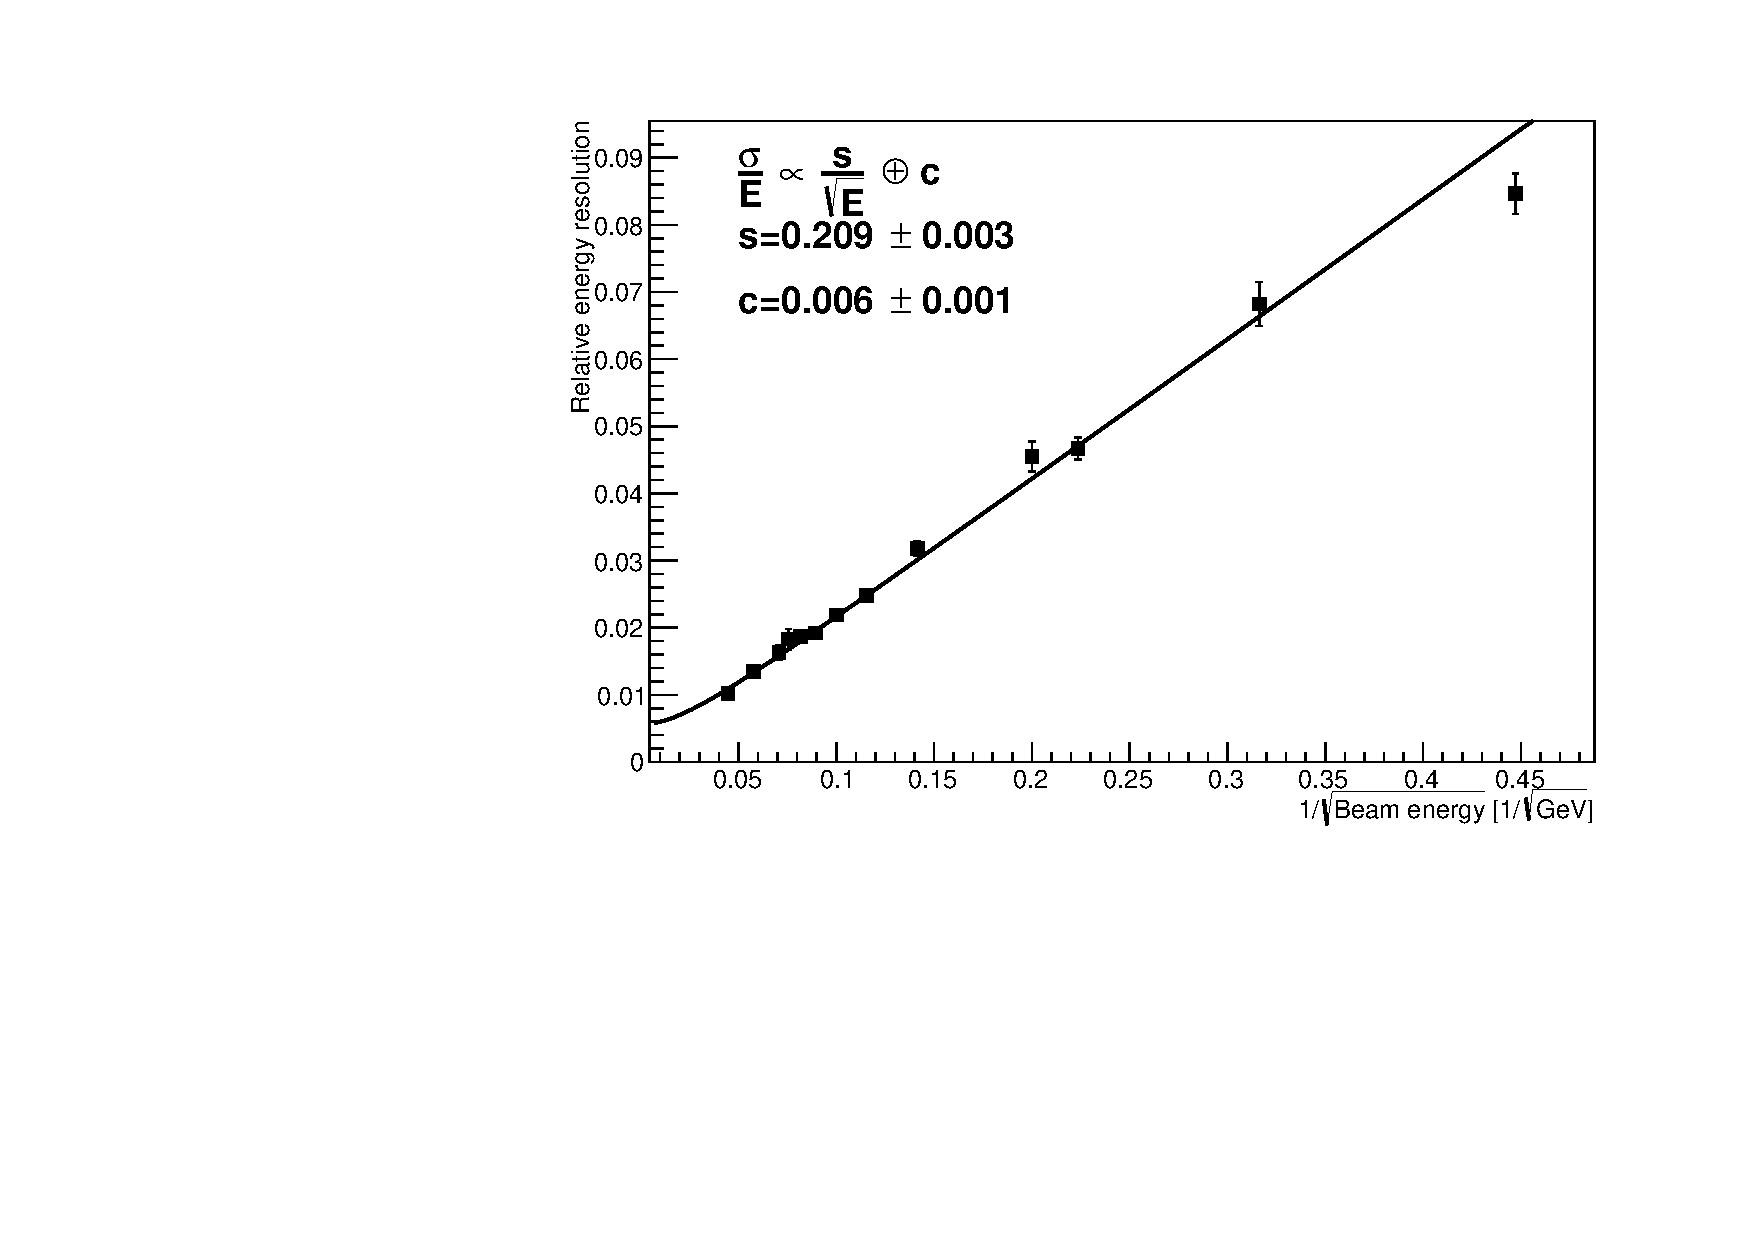
\includegraphics[width=0.48\textwidth]{figures/e_resoFit}
    \caption{{\em Left}: reconstructed energy (in MIP units) as a function of the generated
      energy E. {\em Right}: energy resolution as a function of
      $\frac{1}{\sqrt{E}}$. In both cases single electron events are simulated.}
    \label{fig:baselinelinandresol}
  \end{center}
\end{figure}

Figure~\ref{fig:longprofiles} summarizes the average energy profile
(and energy fluctuation) of the showers for different incident
energies.
The plot on the {\em left} is shown as function of the transversed
thickness transversed in the detector.
It can be observed that for incident energies below 5\GeV the shower
maximum will occur in average in the first section of the detector.
For energies up to 500\GeV the shower maximum will be contained in the
second section of the detector.
As explained above, the fitted longitudinal shower profile to each
event can be used as the estimator of the shower maximum. This
estimator can be used to re-map the energy deposits as function of the
distance to the shower maximum yielding the so-called centered shower
profile shown at the {\em center} of the figure.
This depicts the scaling property of the energy generated by shower
which yields the linear behaviour of the energy estimators used above.
The centered shower profile can be furthermore used to profile the
average fluctuations. This is shown on the {\em right}.
The core of the shower is, has expected, less prone to statistical
fluctuations with an intrinsic resolution of $\approx$10-15\% for
$E>50\GeV$.
The initial stage is prone to the largest fluctuations and the fine
sampling at these earlier stages may therefore provide additional handle on the energy
resolution. This will be discussed later in Section~\ref{sec:optim}.
The last part of the shower, as it will be shown next, is expected to
be dominated by the halo of the shower and, again, is prone to larger
statistical fluctuations with respect to the central region.

\begin{figure}[h!]
  \begin{center}
   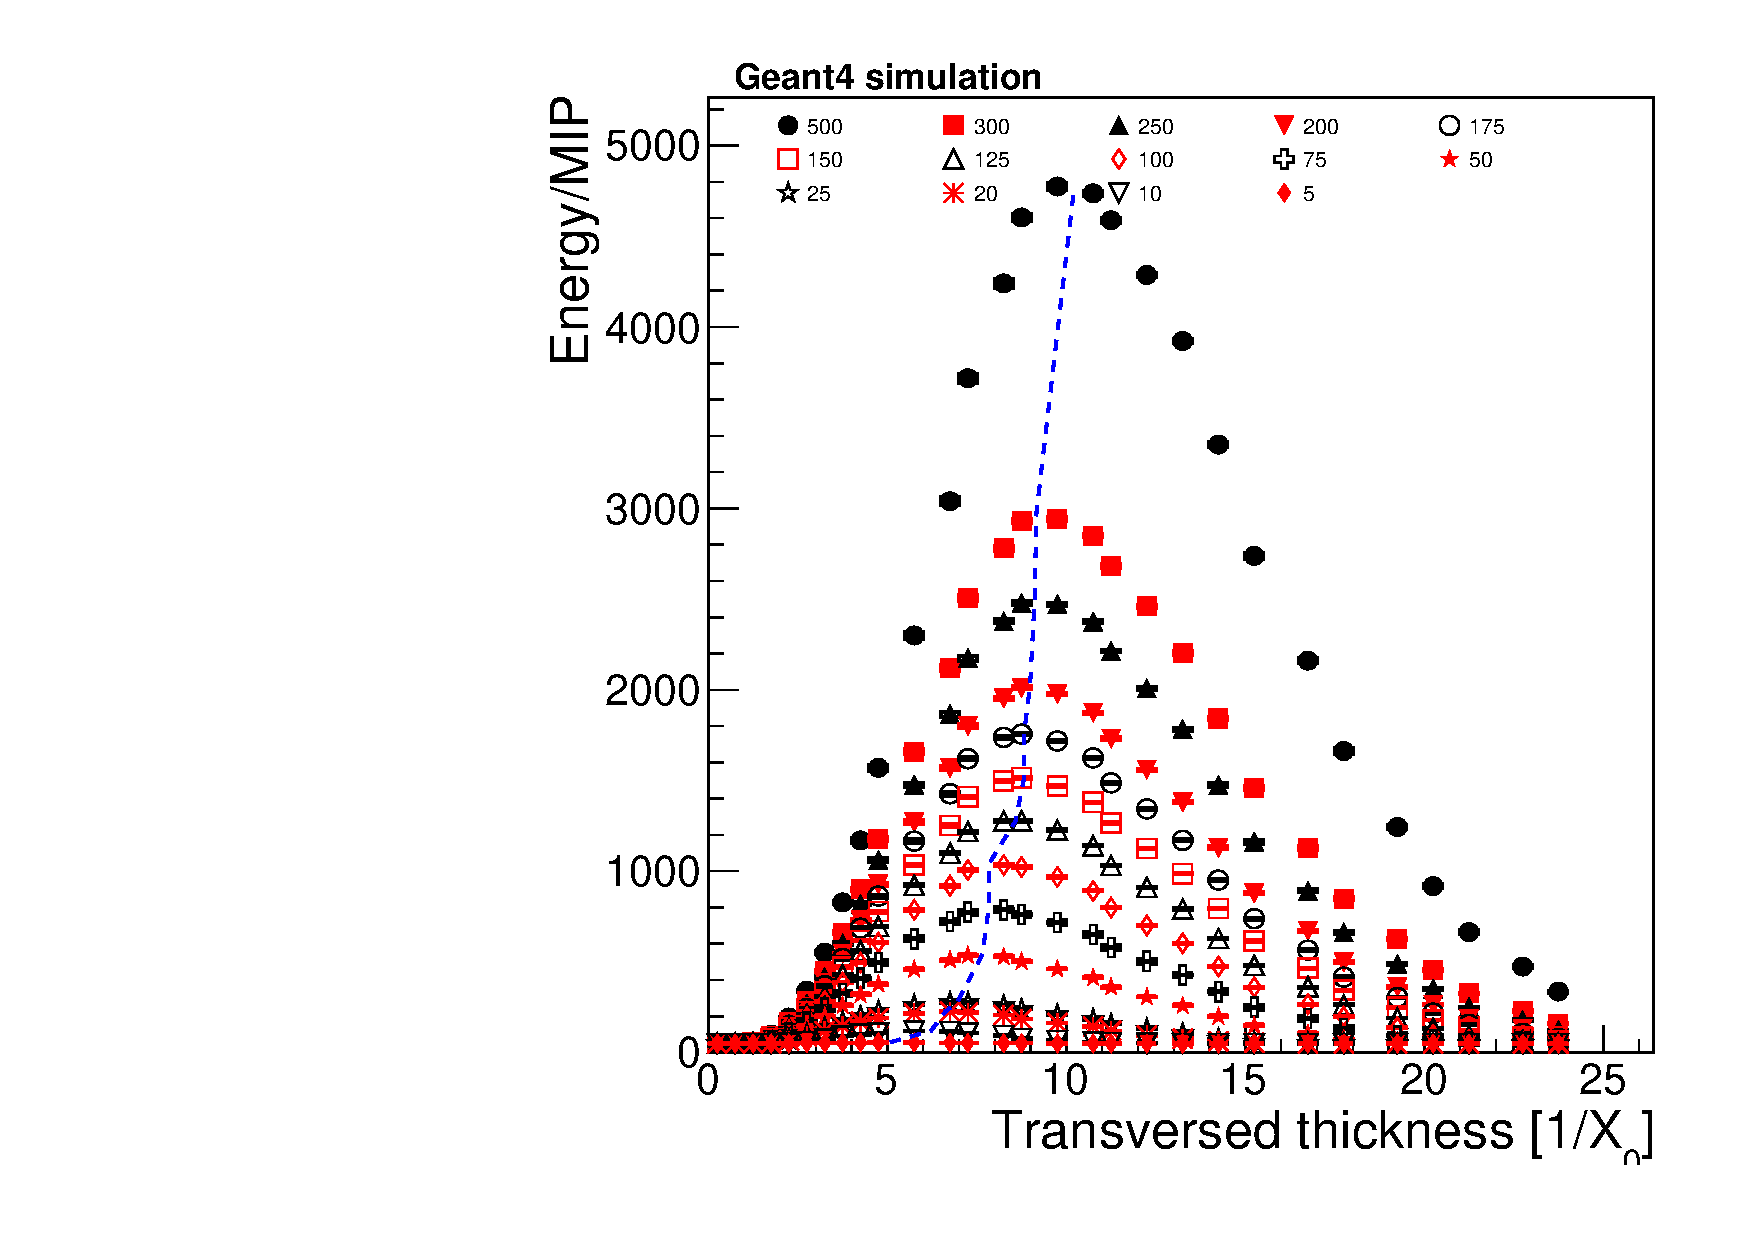
\includegraphics[width=0.32\textwidth]{figures/version_3_rawprof}
    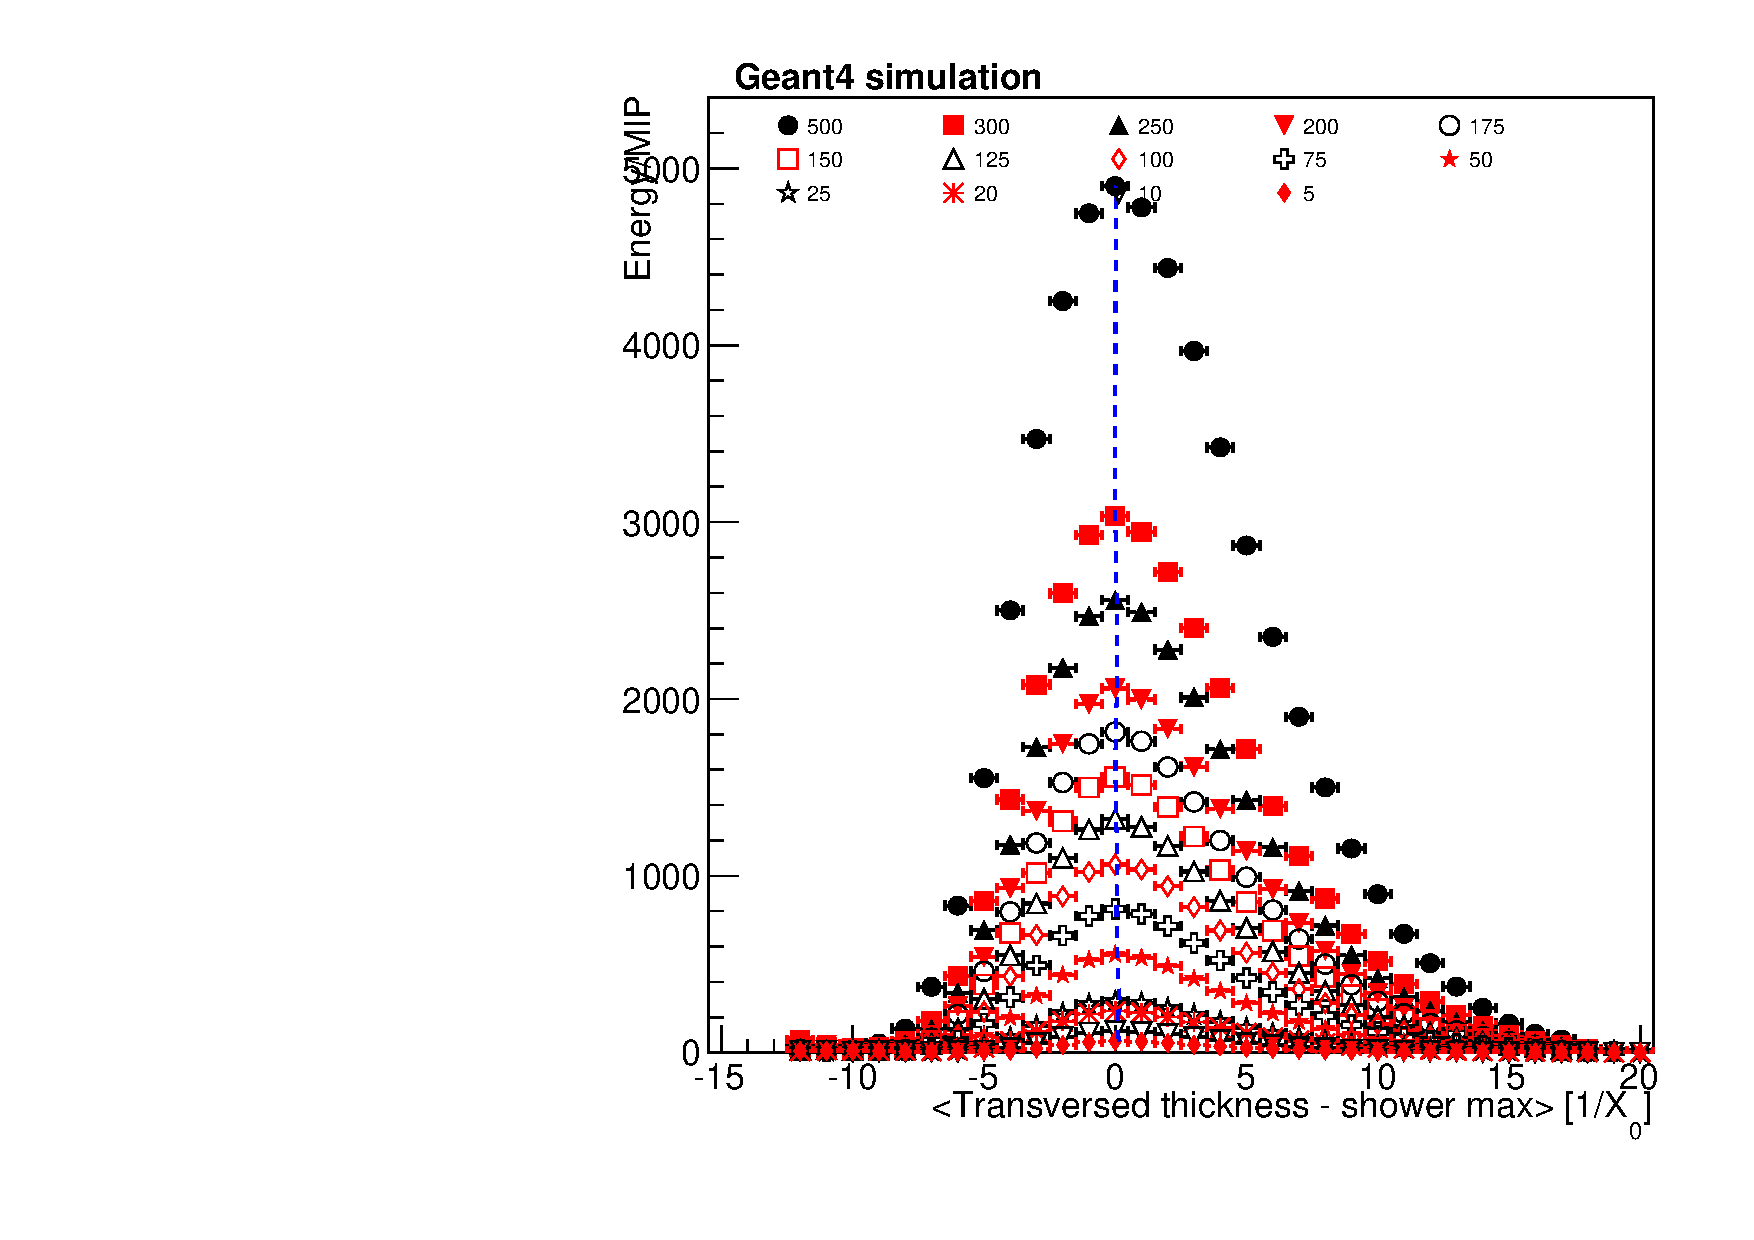
\includegraphics[width=0.32\textwidth]{figures/version_3_cenprof}
    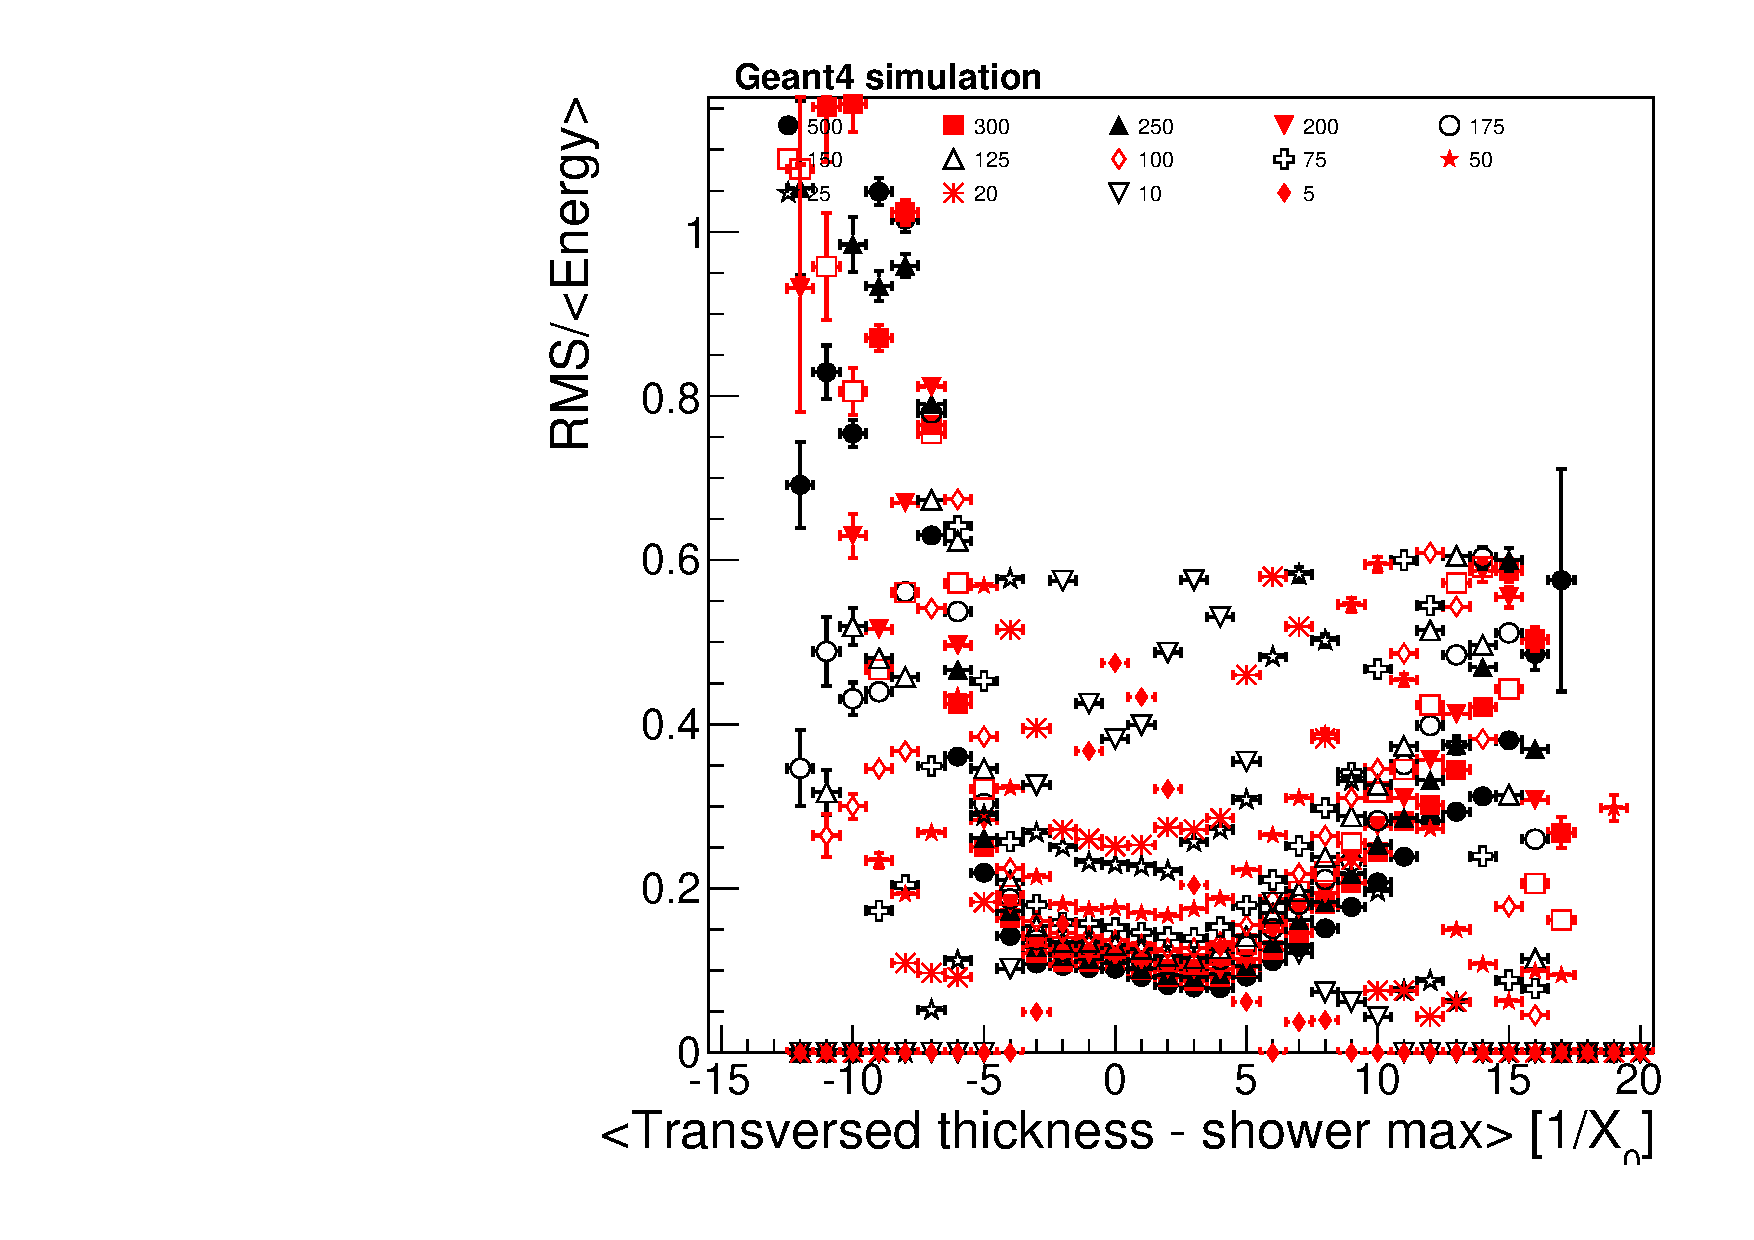
\includegraphics[width=0.32\textwidth]{figures/version_3_crelunc}
    \caption{{\em Left}: average energy deposited as function of the
      transversed thickness in the calorimeter. A blue curve connects
      the estimated shower maximum.
     {\em Center}: average energy deposited as function of the distance
     to the shower maximum estimated on an event-per-event basis.
    {\em Right}: average relative width of the energy deposits as
    function of the distance to the shower maximum estimated on an event-per-event basis.
   }
    \label{fig:longprofiles}
  \end{center}
\end{figure}

%%
%%
%%
\subsection{Transverse shower evolution and shower containment}
\label{subsec:transvevol}

\FIXME{Describe transverse shower properties and Moliere radius}
